\documentclass[a4paper,11pt,final]{book}
\usepackage{fontspec}
\usepackage[czech]{babel}
\usepackage{csquotes}

\AtBeginDocument{\renewcommand\vec{\mathbf}}
\usepackage{amsmath}
\usepackage{unicode-math}  % Fix some weird behaviour (like space before beta)
\usepackage{physics}
\usepackage[version=4]{mhchem}
\usepackage{siunitx}
\sisetup{
	locale               = DE,
	inter-unit-product   = \ensuremath{{}\cdot{}},
	per-mode             = single-symbol,
	list-units           = single,
	list-separator       = {; },
	list-final-separator = \text{ a },
	list-pair-separator  = \text{ a },
	range-phrase         = \text{ až },
	range-units          = single,
}
% Silence warning about conflict of siunitx and physics
\ExplSyntaxOn
\msg_redirect_name:nnn { siunitx } { physics-pkg } { none }
\ExplSyntaxOff

\usepackage{color}
\usepackage{graphicx}
\graphicspath{
	{../efish/}
	{../lif/}
	{../img/}
	{build/epstopdf}
	{img/}
}
\usepackage[outdir=build/epstopdf/]{epstopdf}
\usepackage{tikz}
\usepackage[european, cuteinductors]{circuitikz}

% Tables
\usepackage{caption}
\captionsetup[table]{position=above}
\usepackage{tabularx}                                  % Used in frontmatter
\usepackage{booktabs}
\usepackage{pgfplotstable}
\pgfplotsset{compat=1.17}
\pgfplotstableset{
	use comma,
	set thousands separator = {},
}

\usepackage[hidelinks,pdfusetitle]{hyperref}

\usepackage[style=iso-numeric, autocite=superscript, backend=biber,
	sorting=none, sortlocale=cs_CZ,
	maxcitenames=1, mincitenames=1]{biblatex}
\addbibresource{references.bib}
% Use brackets around superscript references
\DeclareCiteCommand{\supercite}[\mkbibsuperscript]{%
	\iffieldundef{prenote}
	{}
	{\BibliographyWarning{Ignoring prenote argument}}%
	\iffieldundef{postnote}
	{}
	{}%
}
{\bibopenbracket%
	\usebibmacro{citeindex}%
	\usebibmacro{cite}%
	\usebibmacro{postnote}%
	\bibclosebracket}
{\supercitedelim}{}

% Enable including PDF pages (needed for assignment)
\usepackage{pdfpages}

\usetikzlibrary{arrows.meta}
\usetikzlibrary{bending}
\usetikzlibrary{positioning}

\tikzset{
	level/.style = {},
	transition/.style = {
		thick,
		arrows = {-Latex},
	}
}

\DeclareSIUnit\sccm{sccm}
\DeclareSIUnit\arbunit{rel.\ j.}

\newcommand\eu{e}
\newcommand\im{i}

\newcommand\lightspeed{c}
\newcommand\planck{h}

\newcommand\efishsetup{
}

\newcommand\kryptontalifgrotrian{
	\draw [level] (4,0) -- (6,0)
		node [right] {$\mathrm{4p^6\ {}^1S_0}$};
	\draw [level] (4,10) -- (6,10)
		node [right] {$\mathrm{5p'\ [3/2]_2}$};
	\draw [level] (3,6) -- (1,6)
		node [left] {$\mathrm{5s'\ [1/2]_1}$};

	\draw [transition] (5,0) -- (5,5);
	\draw [transition] (5,5) -- (5,10);
	\path (5,0)
		-- node [sloped, below] {$2 \times \SI{204.13}{\nano\metre}$} (5,10);
	\draw [transition] (5,10)
		-- node [sloped, above] {$\SI{826.3}{\nano\metre}$} (2,6);
}

\newcommand\lifgrotrian{
	\draw [level] (4,0) -- (6,0)
		node [right] {$1$};
	\draw [level] (4,10) -- (6,10)
		node [right] {$3$};
	\draw [level] (3,6) -- (1,6)
		node [left] {$2$};

	\draw [transition] (5,0) -- (5,10);
	\path (5,0)
		-- node [sloped, below] {laserová excitace} (5,10);
	\draw [transition] (5,10)
		-- node [sloped, above] {LIF} (2,6);
}

\newcommand\seleniumlifgrotrian{
	\draw [level] (4,0) -- (6,0)
		(5,-1) node {$4s^2 4p^4\ {}^3\mathsf{P}_2$};
	\draw [level] (4,10) -- (6,10)
		(5,11) node {$4s^2 4p^3({}^4\mathsf{S}^o) 5s\ {}^3\mathsf{S^o}_1$};
	\draw [level] (3,6) -- (1,6)
		node [left] {$4s^2 4p^4\ {}^1\mathsf{S}_0$};

	\draw [transition] (5,0) -- (5,10);
	\path (5,0)
		-- node [sloped, below] {\SI{196.09}{\nano\metre}} (5,10);
	\draw [transition] (5,10)
		-- node [sloped, above] {\SI{350.25}{\nano\metre}} (2,6);
}


\def\thetitle{Diagnostika plazmatu pomocí pikosekundového laseru}
\def\thedate{2024}
\def\theauthor{Jan Slaný}

\title\thetitle
\date\thedate
\author\theauthor


\begin{document}

\frontmatter
\pagestyle{empty}

% Title page
\sffamily
\begin{center}
	\includegraphics{logo-muni}
\end{center}
\begin{center}
	\huge Přírodovědecká fakulta
\end{center}
\hrule
\vfill

\begin{flushleft}
\huge\noindent
\textbf{\thetitle}
\end{flushleft}
\bigskip

\large\noindent
Diplomová práce
\bigskip

\Large\noindent
\theauthor
\vfill

\Large\noindent
Vedoucí práce: doc. Mgr. Pavel Dvořák, PhD.
\bigskip

\Large\noindent
Ústav fyzikální elektroniky
\hfill
Brno, 2022

\normalsize
\rmfamily
\cleardoublepage

% Bibliographic entry
\def\bibentryspacing{2}
\chapter*{Bibliografický záznam}
\thispagestyle{empty}
\bgroup
\renewcommand{\arraystretch}{\bibentryspacing}
\begin{tabularx}{\textwidth}{l X}
	\textbf{Autor}            & \theauthor\par
	                            Přírodovědecká fakulta,
	                            Masarykova univerzita\par
	                            Ústav fyzikální elektroniky \\
	\textbf{Název práce}      & \thetitle \\
	\textbf{Studijní program} & Fyzika \\
	\textbf{Studijní obor}    & Fyzika plazmatu a~nanotechnologií \\
	\textbf{Vedoucí práce}    & doc. Mgr. Pavel Dvořák, PhD. \\
	\textbf{Akademický rok}   & 2022/2023 \\
	\textbf{Počet stran}      & \pageref*{lastpage} \\
	\textbf{Klíčová slova}    & plasma, nelineární optika \\
\end{tabularx}
\egroup
\cleardoublepage
\chapter*{Bibliographic Entry}
\thispagestyle{empty}
\bgroup
\renewcommand{\arraystretch}{\bibentryspacing}
\begin{tabularx}{\textwidth}{l X}
	\textbf{Author}           & \theauthor\par
	                            Faculty of Science, Masaryk University\par
	                            Department of Physical Electronics \\
	\textbf{Title of Thesis}  & Plasma diagnostics by means of a picosecond laser \\
	\textbf{Degree Programme} & Physics \\
	\textbf{Field of Study}   & Plasma Physics and Nanotechnology \\
	\textbf{Supervisor}       & doc. Mgr. Pavel Dvořák, PhD. \\
	\textbf{Academic year}    & 2022/2023 \\
	\textbf{Number of Pages}  & \pageref*{lastpage} \\
	\textbf{Keywords}         & plasma, nonlinear optics \\
\end{tabularx}
\egroup

% Abstract
\chapter*{Abstrakt}
Tato práce se zabývá
\vfill
{\let\clearpage\relax\chapter*{Abstract}}
\thispagestyle{empty}
This thesis deals with

% Assignment
\cleardoublepage
% 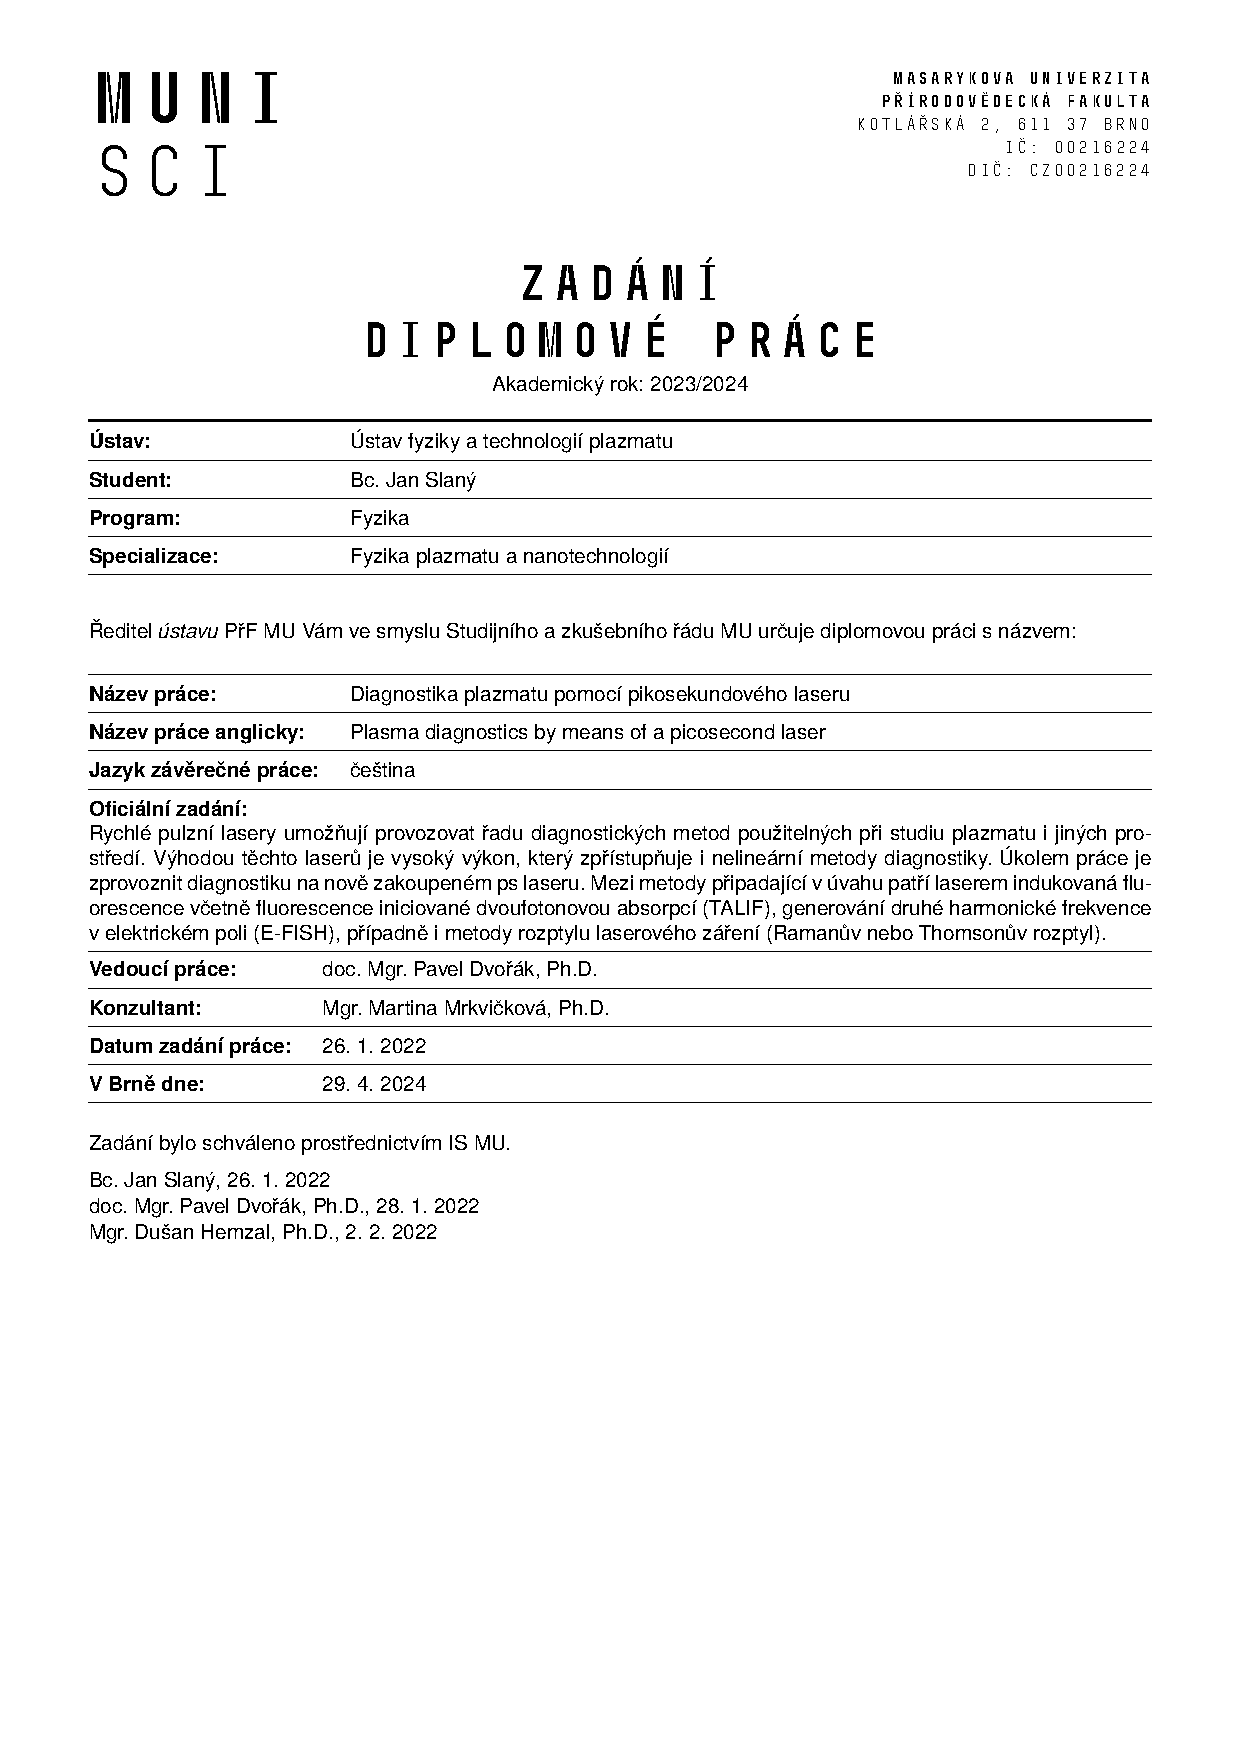
\includepdf[pages={1}]{../zadani.pdf}

% Acknowledgment
\chapter*{Poděkování}
\vfill

% May be on the same page with acknowledgment
{\let\clearpage\relax\chapter*{Prohlášení}}
\thispagestyle{empty}
Prohlašuji, že jsem svou diplomovou práci vypracoval samostatně
pod vedením vedoucího práce s~využitím informačních zdrojů,
které jsou v~práci citovány.
\bigskip

\noindent
V Brně dne 27.~12.~2022
\hfill
\parbox{6cm}{
	\centering
	\vspace{1.5cm}
	\rule{6cm}{0.1pt}\par
	Jan Slaný
}


\mainmatter
\phantomsection\addcontentsline{toc}{chapter}{Obsah}
\tableofcontents
\pagestyle{headings}
% TODO: Úvod
\part{Teoretická část}
\chapter[\EFISH]{Generování druhé harmonické frekvence
	v~elektrickém poli (\EFISH)}
\label{sec:efishth}

\begin{equation}
	\label{eq:efishth-prop}
	\efish \sim A (\alpha^{(3)} \ndens \enlaser \elfield)^2
\end{equation}

\begin{equation}
	\label{eq:efishth-prop-simple}
	\efish \sim (\enlaser \elfield)^2
\end{equation}

\chapter[LIF]{Laserem indukovaná fluorescence}
\label{sec:lifth}
Počátky laserem indukované fluorescence (LIF) sahají do roku 1968,
kdy Richard Zare pomocí \num{632.8}\si{\nano\metre} čáry helium-neonového
laseru analyzoval částice v~draslíkových výparech.
\autocite{lif-original}
Od té doby se s~úspěchem používá ke studiu průhledných médií,
jako jsou plameny nebo plazma.
Ve fyzice plazmatu hraje klíčovou roli při detekci reaktivních částic.
% TODO: \autocite{dvorak1}

Metoda v~sobě spojuje prvky absorpční a~emisní spektroskopie.
Je sice obecně složitejší a~vyžaduje rozsáhlejší a~dražší přístrojové vybavení
než obě tyto metody, ale na oplátku poskytuje několik zásadních výhod.
Mezi nejdůležitější patří nízký detekční limit
a~schopnost detekce nezářivých částic nebo částic s~krátkou dobou života.
Velmi užitečné je také vysoké prostorové rozlišení metody:
Pokud je laserový svazek zaostřen do úzkého profilu a~pozorován z~boku,
je možné získat signál rozlišený ve všech třech prostorových rozměrech.
Při použití krátkopulzního laseru navíc umožňuje výborné časové rozlišení
v~řádu nanosekund až femtosekund.
\autocite{lif-pb}

\section{Princip}
Základní myšlenka metody je pozorování fluorescenčního záření vznikajícího
při deexcitaci zkoumaných částic ze stavu vybuzeného absorpcí laserového
světla.
Obecné schéma nejjednodušší varianty, čítající pouhé tři hladiny,
je na obrázku \ref{fig:lifth-levels}.
Atomy či jiné částice jsou dopadem laseru excitovány ze~základní hladiny~1
do excitovaného stavu~3.
Tento stav je depopulován samovolnou emisí zpět do nižších stavů
(v~tříhladinovém modelu do hladin 1 a~2),
vynucenou emisí do základního stavu způsobenou laserovým zářením
a~řadou dalších procesů probíhajících při srážkách s~okolními částicemi,
které je možno souhrnně nazvat zhášením.
Záření přechodu z~hladiny~3 na hladinu~2 je snímaný fluorescenční signál.

\begin{figure}
	\centering
	\begin{tikzpicture}[scale=0.5]
		\small
		\lifgrotrian
	\end{tikzpicture}
	\caption{Obecné excitační schéma jednofotonové LIF.
		Parametry $\einsteina{i}{j}$ a~$\einsteinb{i}{j}$ jsou Einsteinovy
		koeficienty a~$I$ je intenzita záření.
		Kromě samovolné emise jsou vyšší stavy depopulovány zhášením
		(koeficienty $Q_{ij}$).
		Podle \cite{lif-pb}.}
	\label{fig:lifth-levels}
\end{figure}

\begin{figure}[htb]
	\centering
	\includegraphics[width=\textwidth]{lif-setup-general}
	\caption{Příklad uspořádání experimentu s~LIF.
		Laserový svazek je v~tomto případě pomocí válcových rozptylek
		rozšířen do rovinného tvaru, který je zboku snímán kamerou.
		Podle \cite{lif-oh}.}
	\label{fig:lifth-setup}
\end{figure}

\section{Určení koncentrace částic}
\label{sec:lifth-concentration}
\providecommand\vol{V}
\providecommand\sensabs{D_\text{a}}
\providecommand\lifsens{D_\text{F}}
\providecommand\rayleighsens{D_\text{R}}
\providecommand\lifsignal{M_\text{F}}
\providecommand\rayleighsignal{M_\text{R}}
\providecommand\lifeff{\qeff_\text{F}}
\providecommand\rayleigheff{\qeff_\text{R}}
\providecommand\rayleighdxsect{\dv{\sigma_\text{R}}{\solidangle}}
\providecommand\rayleighndens{\ndens_\text{R}}
\providecommand\enlaserrayleigh{L_\text{R}}
\providecommand\beamprofile{s}
\providecommand\quenching{Q}
\providecommand\liftotal{F}
Velkou výhodou LIF je možnost určit absolutní koncentraci detekovaných částic,
neboť intenzita fluorescence je funkcí této koncentrace.
Závislost je v~limitě nízkých energií laseru lineární,
s~rostoucí energií se pak objevují účinky saturace,
které fluorescenci oslabují (viz dále v~oddíle \ref{sec:lifth-saturation}).

Za předpokladu tříhladinového modelu fluorescenčního procesu uvedeného výše
lze při určování koncentrace vyjít z~rychlostní rovnice popisující
koncentraci horního stavu $\ndens_3$:
\begin{equation}
	\label{eq:lifth-rate-simple}
	\dv{\ndens_3}{\tim}
	= \specoverlap \frac{\einsteinb13 \ity}{\lightspeed} \ndens_1
	- \specoverlap \frac{\einsteinb31 \ity}{\lightspeed} \ndens_3
	- ( \einsteina32 + \quenching_{32} ) \ndens_3,
\end{equation}
kde $\ndens_1$ je koncentrace základního stavu,
$\einsteina{i}{j}$ je Einsteinův koeficient spontánní emise,
$\einsteinb{i}{j}$ jsou Einsteinovy koeficienty absorpce,
$\quenching_{ij}$ je koeficient zohledňující zhášení,
$\ity$ je intenzita ozáření laserem
a~$\lightspeed$ je rychlost světla.
Kromě toho vystupuje ve vztahu také takzvaný
\emph{spektrální překryv} $\specoverlap$,
definovaný pomocí profilu absorpční čáry $a$
a~spektrálního složení laserového záření $l$ normovaných na jedničku:
\begin{equation}
	\label{eq:lifth-specoverlap}
	\specoverlap = \int l(\freq)\,a(\freq) \dd{\freq}.
\end{equation}

Obvykle se mezi základní a~horní hladinou nacházejí další stavy,
které je potřeba do úvahy zahrnout.
Vztah~\eqref{eq:lifth-rate-simple} potom nabývá podoby:
\begin{equation}
	\label{eq:lifth-rate}
	\dv{\ndens_3}{\tim}
	= \specoverlap \frac{\einsteinb13 \ity}{\lightspeed} \ndens_1
	- \specoverlap \frac{\einsteinb31 \ity}{\lightspeed} \ndens_3
	- \left( \sum_i \einsteina3i + \sum_i \quenching_{3i} \right) \ndens_3,
\end{equation}
kde sumy probíhají přes všechny mezilehlé stavy $i$.
Výraz v~závorce udává rychlost úbytku horního stavu všemi samovolnými
procesy (tedy těmi, které nejsou způsobeny laserovým zářením).
Převrácená hodnota této veličiny se nazývá \emph{doba života} $\lifetime$:
\begin{equation}
	\label{eq:lifth-lifetime-def}
	\lifetime = \frac{1}{\sum_i \einsteina3i + \sum_i \quenching_{3i}}.
\end{equation}

Za předpokladu, že se po odeznění laseru vrátí soustava do původního stavu,
musí být celková změna koncentrace $\ndens_3$ rovna nule.
Integrací vzta\-hu~\eqref{eq:lifth-rate} podle času lze tedy získat rovnici:
\begin{equation}
	\label{eq:lifth-rate-int}
	0 = \frac\specoverlap\lightspeed
	\int_0^\infty (\einsteinb13 \ndens_1 - \einsteinb31 \ndens_3) \ity\,\dd\tim
	- \frac1\lifetime \int_0^\infty \ndens_3 \dd{\tim}.
\end{equation}
Celkové množství fluorescenčního záření lze vyjádřit jako:
\begin{equation}
	\label{eq:lifth-liftotal-def}
	\liftotal = \einsteina32 \int_0^\infty \ndens_3 \dd{t}.
\end{equation}
Po dosazení tohoto výrazu do rovnice \eqref{eq:lifth-rate-int}
lze celkové vyzářené množství vyjádřit jako:
\begin{equation}
	\label{eq:lifth-liftotal-general}
	\liftotal = \einsteina32 \lifetime \frac\specoverlap\lightspeed
	\int_0^\infty
	(\einsteinb13 \ndens_1 - \einsteinb31 \ndens_3)
	\ity\,\dd\tim.
\end{equation}
Součin $\einsteina32 \lifetime$ se nazývá kvantový výtěžek a~popisuje,
jaký podíl přechodů se podílí na fluorescenčním záření.

Za předpokladu, že množství stimulované emise do základního stavu
je výrazně menší než absorpce laserového záření
a~že celkové množství popsaných jevů je dostatečně malé, aby mohla být
koncentrace základního stavu $\ndens_1 = \ndens$ považována za konstantní,
lze výraz \eqref{eq:lifth-liftotal-general} zjednodušit následovně:
\begin{equation}
	\label{eq:lifth-liftotal-linear}
	\liftotal \approx \einsteina32 \lifetime
	\frac{\specoverlap\einsteinb13}{\lightspeed}
	\ndens
	\int_0^\infty \ity\,\dd\tim
	\qquad
	\text{kde} \int_0^\infty \ity\,\dd\tim \propto \enlaser,
\end{equation}
kde je možno využít přímé úměry mezi integrálem intenzity
a~energií laserového pulzu $\enlaser$.

Intenzita signálu snímaná v~tomto lineárním režimu je potom
integrálem fluorescenčního záření přes celý objem $\vol$:
\begin{equation}
	\label{eq:lifth-lifsignal}
	\lifsignal = \einsteina32\,\lifetime
	\frac{\specoverlap \einsteinb13}{\lightspeed}
	\ndens \enlaser \lifeff
	\iiint_\vol \sensabs \frac{\solidangle}{4\pi} \beamprofile \dd{\vol},
\end{equation}
kde bylo zavedeno několik parametrů popisujících uspořádání:
$\cameraangle$ je prostorový úhel fluorescenčního záření dopadajícího
na snímač
a~$\beamprofile$ je prostorový profil intenzity laseru normovaný na jedničku.

Citlivost snímače vůči fluorescenčnímu záření ($\lifsens$) obvykle není přímo
známa,
a~byla proto rozepsána jako součin dvou veličin $\lifeff$ a~$\sensabs$.
Relativní citlivost $\lifeff$ je funkcí vlnové délky a~běžně bývá dodávána
výrobcem; mnohdy představuje kvantovou účinnost detektoru.
Absolutní citlivost $\sensabs$ nezávisí na vlnové délce,
ale její hodnota je zpravidla neznámá nebo jen obtížně stanovitelná.

Z~výše uvedeného plyne nutnost při měření zaznamenat nejen samotnou
intenzitu fluorescence $\lifsignal$,
ale také dobu života zářivého stavu $\lifetime$.
Tu je možno změřit z~časového vývoje fluorescenčního záření po odeznění
laserového pulzu,
neboť doba života definovaná vztahem~\eqref{eq:lifth-lifetime-def} vystupuje
jako parametr exponenciálního poklesu intenzity fluorescence v~čase:
\begin{equation}
	\lifsignal \propto \eu^{-\frac{\tim}{\lifetime}}.
\end{equation}
Dobu života lze tedy získat proložením časového vývoje fluorescenčního
signálu exponenciální fukncí.

Větší potíže působí objemový integrál na konci, jehož hodnota není snadno
vyčíslitelná.
Obvykle se proto přistupuje ke kalibraci pomocí Ray\-leigh\-ova rozptylu
ve známém médiu (například vzduchu),
která umožní tento integrál eliminovat.
Měřenou intenzitu Rayleighova rozptylu $\rayleighsignal$ lze popsat vztahem:%
\autocite{lif-oh}
\begin{equation}
	\label{eq:lifth-rayleighsignal}
	\rayleighsignal = \rayleighdxsect \, \rayleighndens
	\frac{\enlaserrayleigh}{\planck\freq} \, \rayleigheff
	\iiint_\vol \sensabs \solidangle \beamprofile \dd{\vol},
\end{equation}
kde $\rayleighndens$ je koncentrace rozptylujících částic,
$\enlaserrayleigh$ je energie laserového pulzu,
$\freq$ je frekvence laserového záření,
$\rayleigheff$ je kvantová účinnost snímače pro použitou vlnovou délku
a~$\rayleighdxsect$ je diferenciální účinný průřez Rayleighova rozptylu.

V~případě vzduchu lze koncentraci částic přibližně vyjádřit pomocí
stavové rovnice ideálního plynu:
\begin{equation}
	\rayleighndens = \frac{\pres}{\boltzmann\temp}.
\end{equation}
Stanovení účinného průřezu $\rayleighdxsect$ je obtížnější,
ale pro běžná média je dobře popsáno v~literatuře.
Rayleighově rozptylu ve vzduchu se věnuje například Miles v~\cite{rayleigh},
kde udává hodnoty indexu lomu a~diferenciálního účinného průřezu vzduchu
pro vlnové délky v~rozsahu \SIrange{200}{1000}{\nano\metre}.

Kombinace vztahů \eqref{eq:lifth-lifsignal} a~\eqref{eq:lifth-rayleighsignal}
vede (v~lineárním režimu) na následující vyjádření koncentrace částic,
kde již objemový integrál nevystupuje:
\begin{equation}
	\label{eq:lifth-ndens}
	\ndens = \frac{\lifsignal}{\rayleighsignal}
	\frac{\enlaserrayleigh}{\enlaser}\frac{\rayleigheff}{\lifeff}
	\frac{1}{A_{32}\,\tau}
	\frac{\lightspeed}{\planck\freq\specoverlap B_{13}}
	\, 4\pi \rayleighdxsect \frac{p}{kT}.
\end{equation}

\section{Saturace}
\label{sec:lifth-saturation}
Podmínky pro dosažení lineárního režimu však nemusejí být vždy splněny.
Při zvýšení intenzity laseru nad určitou hodnotu přestanou platit oba
výše uvedené předpoklady:
Začne se projevovat vyčerpání základní hladiny $\ndens_1$
a~laserem stimulovaná emise zpět do základního stavu nabude nezanedbatelné
hodnoty.
Dostatečná energie laseru navíc může vést k~fotoionizaci excitovaného stavu.
Konečným důsledkem je, že intenzita fluorescenčního záření je nižší,
než předpovídá lineární model.
Tomuto jevu se říká saturace.

Saturace ztěžuje vyhodnocení experimentálních dat, neboť pro stanovení
koncentrace již není možno použít výše popsaný lineární model
a~odvozený vztah~\eqref{eq:lifth-ndens}.
Existují však možnosti, jak jej pro saturaci korigovat.

\Citeauthor{lif-saturation} odvodili v~roce \citeyear{lif-saturation}
následující vztah pro přibližný popis částečně saturovaného
fluorescenčního jevu\autocite{lif-saturation}:
\begin{equation}
	\liftotal(\enlaser) = \frac{\lifslope\enlaser}{1 + \lifsat\enlaser}.
\end{equation}
Zde $\lifslope\enlaser$ je hypotetická fluorescence bez účinků saturace
a~$\lifsat$ je takzvaný saturační parametr.
V~navazující studii z~roku \citeyear{lif-pb} uvádí \citeauthor{lif-pb},
že saturaci lze ve vztahu \eqref{eq:lifth-ndens} zohlednit,
pokud se podíl $\lifsignal/\enlaser$ nahradí vhodným výrazem
závisejícím na konkrétním provedení experimentu.
Zároveň doplňuje příklady pro dvě nejběžnější uspořádání.%
\autocite{lif-pb}

Pro úzký rovinný svazek pozorovaný z~kolmého směru má výraz tvar:
\begin{equation}
	\label{eq:lifth-sheet}
	\liftotal = \frac{2\lifslope}{\lifsat}
	\left( 1 - \frac{\ln(1 + \lifsat\enlasery)}{\lifsat\enlasery} \right),
\end{equation}
kde $\enlasery$ je lineární hustota laserové energie podél osy $y$.
Pro osově souměrný gaussovský svazek nabývá výraz podoby:
\begin{equation}
	\label{eq:lifth-cylindric}
	\liftotal = \frac{\lifslope}{\lifsat}
	\ln(1 + \lifsat\enlaser),
\end{equation}
kde $\enlaser$ je celková energie laserového pulzu.

\part{Experimentální část}
\chapter{Přístrojové vybavení}
\label{sec:instruments}
Na úvod experimentální části je vhodné popsat konkrétní přístroje
a~další součásti používané při pokusech,
neboť některé se opakují ve více aparaturách.

\section{Laser Ekspla \instrname{PL2231-50}}
\label{sec:instruments-laser}
Ústřední součástí všech prováděných pokusů byl samozřejmě laser.
Vždy bylo použito totéž zařízení, konkrétně model \instrname{PL2231-50}
od firmy Ekspla.
Je to diodou čerpaný pevnolátkový pikosekundový laser typu Nd:YAG
poskytující velmi krátké pulzy záření o~vysokém okamžitém výkonu.
Délka pulzu (FWHM) činí \SI{29}{\pico\second}
a~jejich energie může dosahovat až \SI{30}{\milli\joule},
což představuje okamžitý výkon v~řádu \si{\giga\watt}.
Pulzy se opakují s~frekvencí \SI{50}{\hertz}.

\begin{figure}[htp]
	\centering
	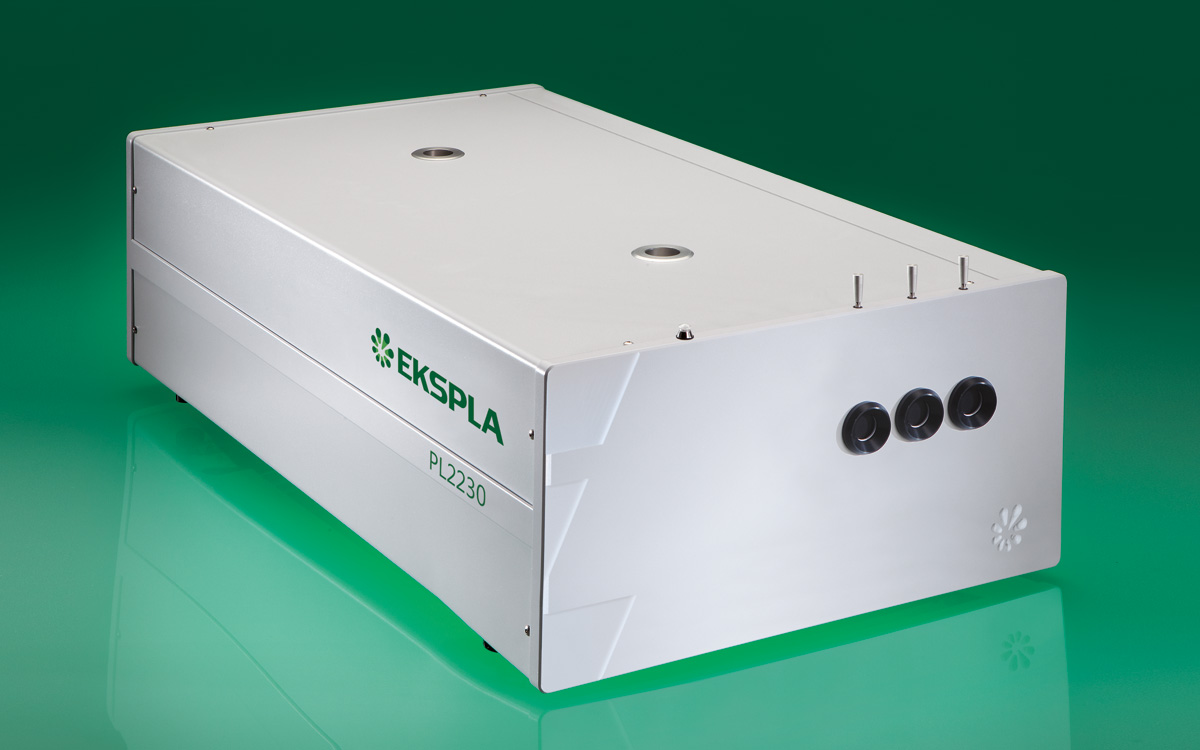
\includegraphics[width=\textwidth]{laser}
	\caption{Pikosekundový laser Ekspla (fotografie z~katalogu).
		Použitý model je ze stejné řady.
		Převzato z~\cite{ekspla-datasheet}.}
	\label{fig:instruments-laser}
\end{figure}

Aktivním médiem je krystal yttrito-hlinitého granátu (\ce{Y3Al5O12})
dopovaný ionty neodymu (\ce{Nd3+}).\autocite{wiki-ndyag}
Základní vlnová délka laseru je \SI{1064}{\nano\metre},
stejně jako pro všechny lasery typu Nd:YAG,
jeho součástí jsou ale teplotně stabilizované jednotky obsahující
krystaly di\-hydro\-gen\-fosfo\-rečnanu draselného (KDP a~KD*P),
které umožňují generování druhé, třetí a čtvrté harmonické frekvence,
tedy vlnových délek \SIlist{532; 355; 266}{\nano\metre}.
\autocite{ekspla-datasheet}

Generování začíná v~hlavním pevnolátkovém oscilátoru čerpaném diodami,
který vytváří řetězce pulzů s~frekvencí opakování jednotlivých pulzů
přibližně \SI{87}{\mega\hertz} (tzv.~\emph{trains}).
Pulzy jsou slabé, jejich energie se pohybuje v~jednotkách \si{\nano\joule}.
Tyto putují do diodového regenerativního zesilovače se zesílením v~řádu $10^6$
a~poté do víceprůchodového výkonového zesilovače,
takže jejich konečná energie je kolem $\SI{30}{\milli\joule}$.
Výstupní energie je nastavitelná v~krocích po zhruba \SI{1}{\percent}
a~je velmi stabilní mezi po sobě jdoucími pulzy
(odchylky jsou menší než \SI{0.5}{\percent} středního kvadratického průměru
při nastavené základní vlnové délce).
\autocite{ekspla-datasheet}

Výstupní profil laserového svazku je podle výrobce přibližně gaussovský
(viz obrázek~\ref{fig:instruments-beamprofile})
o~průměru cca \SI{6}{\milli\metre} na úrovni $1/e^2$ maxima
pro vlnovou délku \SI{1064}{\nano\metre}.
\autocite{ekspla-datasheet}
Navzdory těmto specifikacím se ukázalo, že profil svazku je závislý
na nastavené energii pulzu v~míře, kterou nelze zanedbat.
Tato problematika je podrobněji popsána v~dalších kapitolách,
viz především oddíl \ref{sec:lif-rayleigh}.

Laser je vybaven vlastním měřičem, který průběžně zaznamenává energii pulzu.
K~synchronizaci dalších zařízení slouží spouštěcí signál s~nastavitelným
předstihem.\autocite{ekspla-datasheet}

\begin{figure}[htp]
	\centering
	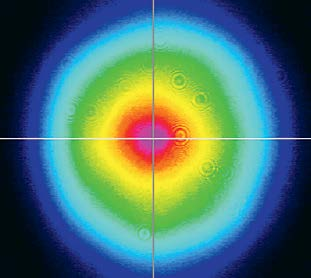
\includegraphics[scale=0.5]{ekspla-beamprofile}
	\caption{Typický profil laserového svazku v~blízkém poli
		uvedený v~technickém listu laseru.
		Převzato z~\cite{ekspla-datasheet}.}
	\label{fig:instruments-beamprofile}
\end{figure}

\section{ICCD kamera \instrname{Pimax}}
\label{sec:instruments-iccd}

\begin{figure}[htp]
	\centering
	\input{img/cameraeff}
	\caption{Kvantová účinnost kamery deklarovaná výrobcem.}
	\label{fig:instruments-cameraeff}
\end{figure}

\chapter[\EFISH]{{\EFISH} v~dielektrickém bariérovém výboji}

\newcommand\ypos{y}

\section{Úvod}
\label{sec:efish-intro}
Experiment popsaný v~této kapitole byl jeden z~vůbec prvních pokusů
provedených na novém pikosekundovém laseru po jeho instalaci.
Jeho záměrem bylo pozorovat generování druhé harmonické frekvence
a~využít je k~určení intenzity elektrického pole v~dielektrickém
bariérovém výboji.
%
Druhotným úkolem bylo ověření možností, které laser nabízí.

Výsledky tohto pokusu byly ještě před dokončením práce publikovány
T.~Hoderem et al.~v~článku \cite{efish-nitrogen}, na nějž se dovolujeme
odkazovat.

\section{Uspořádání experimentu}
\label{sec:efish-setup}
Měření bylo uskutečněno na téže aparatuře, jako je popsána
v~\cite{efish-nitrogen},
následující odstavce jsou proto parafrázovány odtamtud.

Předmětem zkoumání byl Townsendův výboj v~dusíku za atmosférického tlaku.
Výboj byl v~dielektrickém bariérovém uspořádání, které ukazuje
obrázek~\ref{fig:efish-reactor}.
Rovinné elektrody o~rozměrech \num{14}\times\SI{15}{\milli\metre}
jsou naneseny na dvou podložních sklíčkách tloušťky \SI{1.1}{\milli\metre}.
Jejich materiálem je sklo s~relativní permitivitou ${\relperm = \num{4.7}}$.
Mezi sklíčky je mezera o~šířce zhruba \SI{1}{\milli\metre}.
Zařízení je umístěno vodorovně v~uzavřeném plastovém reaktoru.
Čistý dusík je přiváděn otvorem v~rovině výboje v~boční stěně reaktoru
a~odváděn podobným otvorem naproti.

Reaktor je vybaven dvěma okénky z~křemenného skla umístěnými naproti
sobě v~úrovni výboje,
která umožňují přímé pozorování a~laserovou diagnostiku.
Okénka jsou skloněna dolů pod Brewsterovým úhlem, aby byl minimalizován
odraz laserového svazku (který je svisle polarizovaný).

Výboj je napájen střídavým napětím o~frekvenci \SI{11}{\kilo\hertz}
a~amplitudě kolem \SI{6}{\kilo\volt},
které je dále modulováno \num{500}\si{\hertz} čtvercovým signálem
se střídou \SI{45}{\percent}.
Výsledkem je deset napěťových cyklů o~celkové délce \SI{909}{\milli\second}
následovaných \SI{1091}{\milli\second} nulového napětí.
\autocite{efish-nitrogen}
Část modulačního cyklu je na obrázku~\ref{fig:efish-overview-full},
detail jednoho napěťového cyklu je na obrázku~\ref{fig:efish-overview-period}.

Schéma optické dráhy je na obrázku~\ref{fig:efish-setup}.
Laser je nastavený na základní frekvenci \SI{1064}{\nano\metre}.
Svazek je zaostřen spojkou o~ohniskové vzdálenosti \SI{50}{\milli\metre}
do středu výbojového prostoru v~reaktoru skrz první okénko.
Mezi elektrodami dochází ke generování druhé harmonické frekvence
(vlnové délky \SI{532}{\nano\metre}), která společně s~původním svazkem
vystupuje druhým okénkem ven.
Zde jsou frekvence od sebe odděleny pomocí dichroického zrcátka,
které harmonickou složku odráží a~základní propouští.
Odražený svazek je po kolimaci druhou spojkou dále očištěn od nežádoucích
složek pomocí druhého dichroického zrcátka a~disperzního hranolu.

Intenzitu harmonického svazku (tedy signál \EFISH{})
měří mikrokanálový fotonásobič
Photek \instrname{PMT210} s~průměrem aktivní oblasti \SI{10}{\milli\metre},
pološířkou pulzu (FWHM) \SI{150}{\pico\second} a~zesílením \num{e6}.
Před fotonásobičem je umístěna irisová clona a~úzkopásmový filtr
pro dodatečné filtrování svazku a~odstínění parazitního záření
z~jiných zdrojů.

Energie původního svazku je měřena dvojím způsobem:
Za prvním dichroickým zrcátkem se nachází pyroelektrický měřič energie
Ophir \instrname{PE50BF-DIF}, jenž snímá celkovou energii pulzů.
Kromě toho je u~vstupního okénka reaktoru umístěna fotodioda
Thorlabs \instrname{DET10A/M}, která měří část svazku odraženou na okénku.

Napájecí napětí výboje, procházející proud, intenzita svazku z~fotodiody
a~signál \EFISH{} z~fotonásobiče jsou zaznamenávány osciloskopem
Keysight \instrname{DSO-S204A},
který je vybaven vysokonapěťovou sondou Tektronix \instrname{P6015A}
a~proudovou sondou Tektronix \instrname{CT2}.

\begin{figure}
	\includegraphics[width=\textwidth]{efish-reactor}
	\caption{Uspořádání zkoumaného výboje.
		Komora reaktoru je válcová, přívod a~odvod plynu se nacházejí
		ve směru kolmém k~ose procházející oběma okénky.
		Šířka mezery mezi podložními sklíčky je \SI{1}{\milli\metre}.
		Podle \cite{efish-nitrogen}.}
	\label{fig:efish-reactor}
\end{figure}

\begin{figure}
	\includegraphics[width=\textwidth]{efish-setup}
	\caption{Uspořádání celého experimentu.
	První spojka zaostřuje svazek do středu výbojového prostoru
	uvnitř reaktoru.
	Druhá spojka slouží ke kolimaci svazku.
	Dichroická zrcátka odrážejí druhou harmonickou frekvenci
	a~propouštějí základní.
	Energie laserového pulzu je snímána fotodiodou i~měřičem energie.
	Před fotonásobičem je filtr propouštějící pouze úzkou oblast
	kolem druhé harmonické frekvence.
	Podle \cite{efish-nitrogen}.}
	\label{fig:efish-setup}
\end{figure}

\begin{figure}[htp]
	\centering
	\input{../efish/results/overview-full}
	\caption{Průběh napětí na elektrodách a~proudu ve výboji
		za několik cyklů.}
	\label{fig:efish-overview-full}
	\vspace{24pt}
	\input{../efish/results/overview-period}
	\caption{Detail jednoho cyklu výboje.}
	\label{fig:efish-overview-period}
\end{figure}

\section{Ověření opakovatelnosti}
\label{sec:efish-check}
Protože laserová aparatura byla v~době měření zcela nová,
bylo vhodné před samotným pokusem ověřit některé charakteristiky
laserových pulzů a~signálu \EFISH{},
zejména opakovatelnost s~konstantní intenzitou a~tvarem,
která je nezbytná k~získání věrohodných výsledků.

Opakovatelnost laserového pulzu byla ověřena změřením sta jednotlivých
snímků (tj.~bez akumulací na osciloskopu) za stálých podmínek.
Laser byl nastaven na konstantní zesílení i~vlnovou délku
a~napájení výboje na konstantní amplitudu napětí.
Intenzita svazku odraženého z~okénka, zachycená fotodiodou,
měla stabilní tvar i~amplitudu, jak ukazuje
obrázek~\ref{fig:efish-pulse-compare}.

Stabilita signálu \EFISH{} byla rovněž dobrá.
Obrázek~\ref{fig:efish-singleshots-compare} ukazuje signál
\EFISH{} změřený fotonásobičem v~průběhu téhož měření,
tedy jednotlivé snímky bez akumulací.
Je vidět, že tvar hlavního pulzu je velmi podobný ve všech snímcích,
šířka je stálá a~náběhová hrana má stejný sklon.
V~některých případech se mírně liší amplituda.

\begin{figure}[htp]
	\centering
	\input{../efish/results/pulse-compare}
	\caption{Ověření konstantnosti laserového pulzu.
		Zobrazena je intenzita laserového svazku odraženého
		na okénku reaktoru zaznamenaná fotodiodou.
		Jedná se o~jednotlivé snímky bez akumulací v~osciloskopu.
		Laser je nastaven na stabilní zesílení.
		Pro přehlednost je zobrazen pouze výběr snímků.}
	\label{fig:efish-pulse-compare}
\end{figure}

\begin{figure}[htp]
	\centering
	\input{../efish/results/singleshots-compare}
	\caption{Ověření reprodukovatelnosti signálu \EFISH{} zachyceného
		fotonásobičem.
		Výběr ze sta snímků zaznamenaných osciloskopem bez průměrování.
		Opakovatelnost se zdá být dostatečná,
		tvar hlavního pulzu je velmi podobný ve všech snímcích.}
	\label{fig:efish-singleshots-compare}
\end{figure}

Vztah mezi signálem z~fotodiody (tj.~intenzitou laseru)
a~fotonásobiče (signálem \EFISH{}) ilustruje
obrázek~\ref{fig:efish-singleshot}.
Je na místě připomenout, že vzájemný časový posun obou signálů
zaznamenaný osciloskopem se~pravděpodobně liší od skutečnosti,
neboť nelze zaručit stejné zpoždění v~obou detekčních cestách.

\begin{figure}[htp]
	\centering
	\input{../efish/results/singleshot}
	\caption{Signál \EFISH{} z~jediného snímku
		a~intenzita laserového pulzu, který jej vyvolal.
		Čas $\tim$ je čas záznamu osciloskopem a~neodpovídá skutečnému času,
		kdy k~ději došlo.
		Zejména není zaručeno, že zpoždění je v~obou případech stejné.}
	\label{fig:efish-singleshot}
\end{figure}

Závislost časového průběhu signálu \EFISH{} na~energii laserového pulzu
je na obrázku~\ref{fig:efish-energy-corrected}.
Je vidět, že tvar je až na absolutní velikost velmi podobný pro všechny
energie.
Malá odchylka se projeví v~poklesové části pulzu, neboť signál způsobený
silnějším pulzem klesá mírně pomaleji než u~slabších.
Tento rozdíl je vidět na obrázku~\ref{fig:efish-energy-norm},
kde jsou data normována tak, aby měla jednotkovou amplitudu signálu.

\begin{figure}[htp]
	\centering
	\input{../efish/results/energy-corrected}
	\caption{Signál \EFISH{} pro různé energie laserového pulzu.}
	\label{fig:efish-energy-corrected}
	\vspace{24pt}
	\input{../efish/results/energy-norm}
	\caption{Signál \EFISH{} pro různé energie pulzu normovaný na stejnou
		amplitudu (\num{-1}).
		Je vidět, že odpovídá tvar hlavního pulzu i~pozadí
		(data jsou korigována odečtením pozadí).
		Největší rozdíly jsou patrny v~poklesové části pulzu.}
	\label{fig:efish-energy-norm}
\end{figure}

\section{Vyhodnocení}
\label{sec:efish-method}

\begin{figure}[htp]
	\centering
	\input{../efish/results/intmax}
	\caption{Korelace intenzity signálu \EFISH{} určené dvěma způsoby:
		Jako maximální hodnota intenzity a~jako integrál intenzity.}
	\label{fig:efish-intmax}
\end{figure}

\section{Výsledky}
\label{sec:efish-results}

\begin{figure}
	\centering
	\input{../efish/results/period-calib-bilateral}
	\caption{Kalibrační funkce použité pro vyhodnocení časového vývoje.
		Funkce ve středu mezery byla změřena dvakrát, poprvé před měřením
		elektrického pole v~dolní části mezery (střed 1)
		a~podruhé před měřením horní části (střed 2).
		Záporná větev je extrapolována z~pravé.
		Označená minima ukazují, že všechny funkce jsou mírně posunuty
		doleva (zhruba o~\SI{0.4}{\mega\volt\per\metre}).}
	\label{fig:efish-period-calib}
\end{figure}

\begin{figure}[htp]
	\centering
	\input{../efish/results/period-efish}
	\caption{Intenzita \EFISH{} zaznamenaná v~různých výškách
		v~průběhu jedné periody budicího napětí.}
	\label{fig:efish-period-efish}
\end{figure}

\begin{figure}[p]
	\sisetup{per-mode = symbol}
	\input{../efish/results/period-elfield}
	\caption{Časový vývoj intenzity elektrického pole
		v~různých místech výboje.
		Spodní elektroda se nachází zhruba ve~výšce
		$\ypos = \SI{-0.35}{\milli\metre}$,
		horní elektroda přibližně ve~výšce
		$\ypos = \SI{0.7}{\milli\metre}$.}
\end{figure}

\begin{figure}[htp]
	\centering
	\input{../efish/results/period-amplitude}
	\caption{Amplituda intenzity elektrického pole určená z~maxima
		a~minima spočteného průběhu v~čase.
		Měření proběhlo ve dvou sériích (kladné a~záporné $\ypos$),
		které se překrývají v~bodě $\ypos = 0$.
		To je příčinou dvojí hodnoty v~tomto bodě.}
	\label{fig:efish-period-amplitude}
\end{figure}

\chapter[LIF]{Laserem indukovaná fluorescence selenu}
\label{sec:lif}

\providecommand\xpos{x}
\providecommand\ypos{y}
\providecommand\xmm{x}
\providecommand\ymm{h}
\providecommand\voigtsigma{\sigma}
\providecommand\voigtgamma{\gamma}
\providecommand\lifslopex{\lifslope_\text{x}}
\providecommand\lifslopet{\lifslope_\text{t}}
\providecommand\lifsatx{\lifsat_\text{x}}
\providecommand\lifsatt{\lifsat_\text{t}}
\providecommand\lifslopeunit{10^9}
\providecommand\lifsatunit{\per\micro\joule}
\providecommand\ndensse{n_\text{Se}}
\providecommand\ndensseunc{\sigma_{\!n,\,\text{Se}}}
\renewcommand\einsteina{A_{32}}
\renewcommand\einsteinb{B_{13}}

\section{Úvod}
\label{sec:lif-intro}
Posledním provedeným experimentem bylo určení absolutní koncentrace
selenu ve vodíkovém plameni pomocí laserem indukované fluorescence.
Ačkoli se může zdát, že se takový pokus vymyká tématu práce,
plamen s~diagnostikou plazmatu stále souvisí.
Spojovacím článkem mezi nimi je atomizace.

Atomizace je rozklad sloučeniny na jednotlivé atomy v~plynné fázi.
V~analytické chemii je to běžně používaný proces sloužící k~určení
koncentrace určitých atomů ve vzorku:
Neznámý vzorek je atomizován a vzniklý plyn je podroben zkoumání,
při němž mnohdy hrají nemalou roli optické metody.

Pro atomizaci se často používá plamene, hledají se však alternativní cesty
jako třeba pomocí plazmatu.
Plamen je široce znám a~podrobně popsán,
slouží proto jako dobré srovnávací médium.
Měření fluorescence v~plameni lze tedy chápat jako referenci
pro fluorescenci v~plazmatu.

\section{Uspořádání experimentu}
\label{sec:lif-setup}

\subsection{Chemická část}
\label{sec:lif-setup-chemistry}
Za zkoumaný vzorek byl použit roztok \SI{10}{\ppb}
(tedy \SI{10}{\micro\gram\per\litre})
selenu v kyselině chlorovodíkové \ce{HCl} o koncentraci \SI{1}{\mol\per\litre}.
Směs proudila do generátoru hydridů, kde byl selen redukován
\num{0.5}\si{\percent} roztokem borohydridu sodného (\ce{NaBH4})
v~\num{0.4}\si{\percent} hydroxidu draselném (\ce{KOH}).
Redukovaný selen následně reagoval s~atomárním vodíkem za vzniku
selanu (tj.~hydridu selenu, \ce{H2Se}).

Selan je těkavá látka, která má za standardních podmínek podobu
bezbarvého plynu.
Ten byl veden do atomizátoru spolu s~nosným plynem argonem
o~průtoku \SI{775}{\sccm}.
Dalším kanálem atomizátoru byl přiváděn vodík o~průtoku \SI{300}{\sccm}.
Nad ústím atomizátoru, kde se vodík mísil s~okolním vzduchem,
hořel vodíkový plamen, v~němž docházelo ve dvou krocích
k~atomizaci selenu rozpadem selanové molekuly \ce{H2Se}:
\begin{align*}
	\ce{
		H + H2Se &-> H2 + HSe \\
		H + HSe &-> H2 + Se
	}
\end{align*}

\begin{figure}
	\centering
	\begin{tikzpicture}[scale=0.5]
		\seleniumlifgrotrian
	\end{tikzpicture}
	\caption{Excitační schéma selenu použité pro LIF.}
\end{figure}

\subsection{Optická část}
\label{sec:lif-setup-optics}
Volba optické dráhy se odvíjela od dvou základních požadavků:
Za prvé bylo potřeba eliminovat nebo alespoň dostatečně potlačit
nehomogennost intenzity laserového svazku,
jejíž profil navíc závisí na nastaveném zesílení laseru.
Za druhé byla celková energie laserových pulzů příliš velká
a~vedla by k~velmi vysokému stupni saturace, potažmo obtížnému vyhodnocení,
pročež bylo nutné ji před vstupem do plamene značně omezit.

Pro zajištění rovnoměrnějšího rozložení intenzity byl laserový svazek
po výstupu ze~zdroje veden do prostorového filtru tvořeného dvěma
křemennými spojkami a~clonou s~kruhovou dírkou. % TODO: polomer
Následně byl svazek rozdělen děličem svazku.
Jako dělič sloužila skleněná destička,
která většinu záření propouštěla do detektoru
a~pouze malou část odrážela dále do aparatury,
čímž došlo k~požadovanému snížení intenzity.

V~dráze odraženého svazku byla umístěna irisová clona za účelem
odstínění parazitního světla.
Při některých měřeních byl kvůli zlepšení prostorového rozlišení
svazek dále ořezán průchodem svislou štěrbinou na rovinný tvar,
takže konečný průřez svazku byl přibližně obdélník
o~výšce \SI{3}{\milli\metre} a~tloušťce \SI{1}{\milli\metre}.
Upravený svazek vodorovně procházel středovou oblastí plamene.
Schéma celého uspořádání je na obrázku č.~\ref{fig:lif-setup}.

Intenzita svazku je měřena dvojicí detektorů
zaznamenávajích energii jednotlivých pulzů.
Svazek procházející děličem putuje přímo do detektoru
Ophir \instrname{Vega Pyroelectric PE9}
s~rozsahem \SIrange{0.2}{1000}{\micro\joule}.
Za~atomizátorem je umístěn citlivější detektor
Ophir \instrname{Vega Pyroelectric PE9-ES-C}
s~rozsahem \SIrange{0.1}{200}{\micro\joule},
který měří svazek procházející plamenem.
Pro velmi nízké energie pulzu je citlivější detektor přesunut
za dělič (kde je svazek silnější) a~svazek za~atomizátorem není měřen.

V~oblasti, kde se křížil laserový svazek s~plamenem, docházelo k~fluorescenci.
Její záření bylo z~boku snímáno ICCD kamerou synchronizovanou s~laserem.
Použitý model kamery byl \instrname{PIMAX-3} od Princeton Instruments.
Citlivost kamery byla zvýšena opakovanou akumulací signálu na čipu.
Počet akumulací pro LIF byl obvykle 100, ale mohl být regulován dle potřeby.
Před kamerou se nacházela dvojice křemenných sklíček,
která sloužila jako filtr pro odstínění parazitního světla.
Snímek skutečného provedení je na obrázku \ref{fig:lif-setup-photo}.

\begin{figure}[htb]
	\centering
	\includegraphics[width=\textwidth]{img/lif-setup-se}
	\caption{Schéma uspořádání experimentu.
		Svazek je na začátku upraven prostorovým filtrem,
		aby se jeho profil více podobal gaussovskému.
		Pro měření je použita jen malá část svazku odražená na skleněné desce,
		zbytek prochází do~prvního měřiče, jenž zaznamenává jeho energii.
		Svislá štěrbina zajišťuje rovinný profil svazku,
		ale nebyla použita ve všech experimentech.}
	\label{fig:lif-setup}
\end{figure}

\begin{figure}[htp]
	\centering
	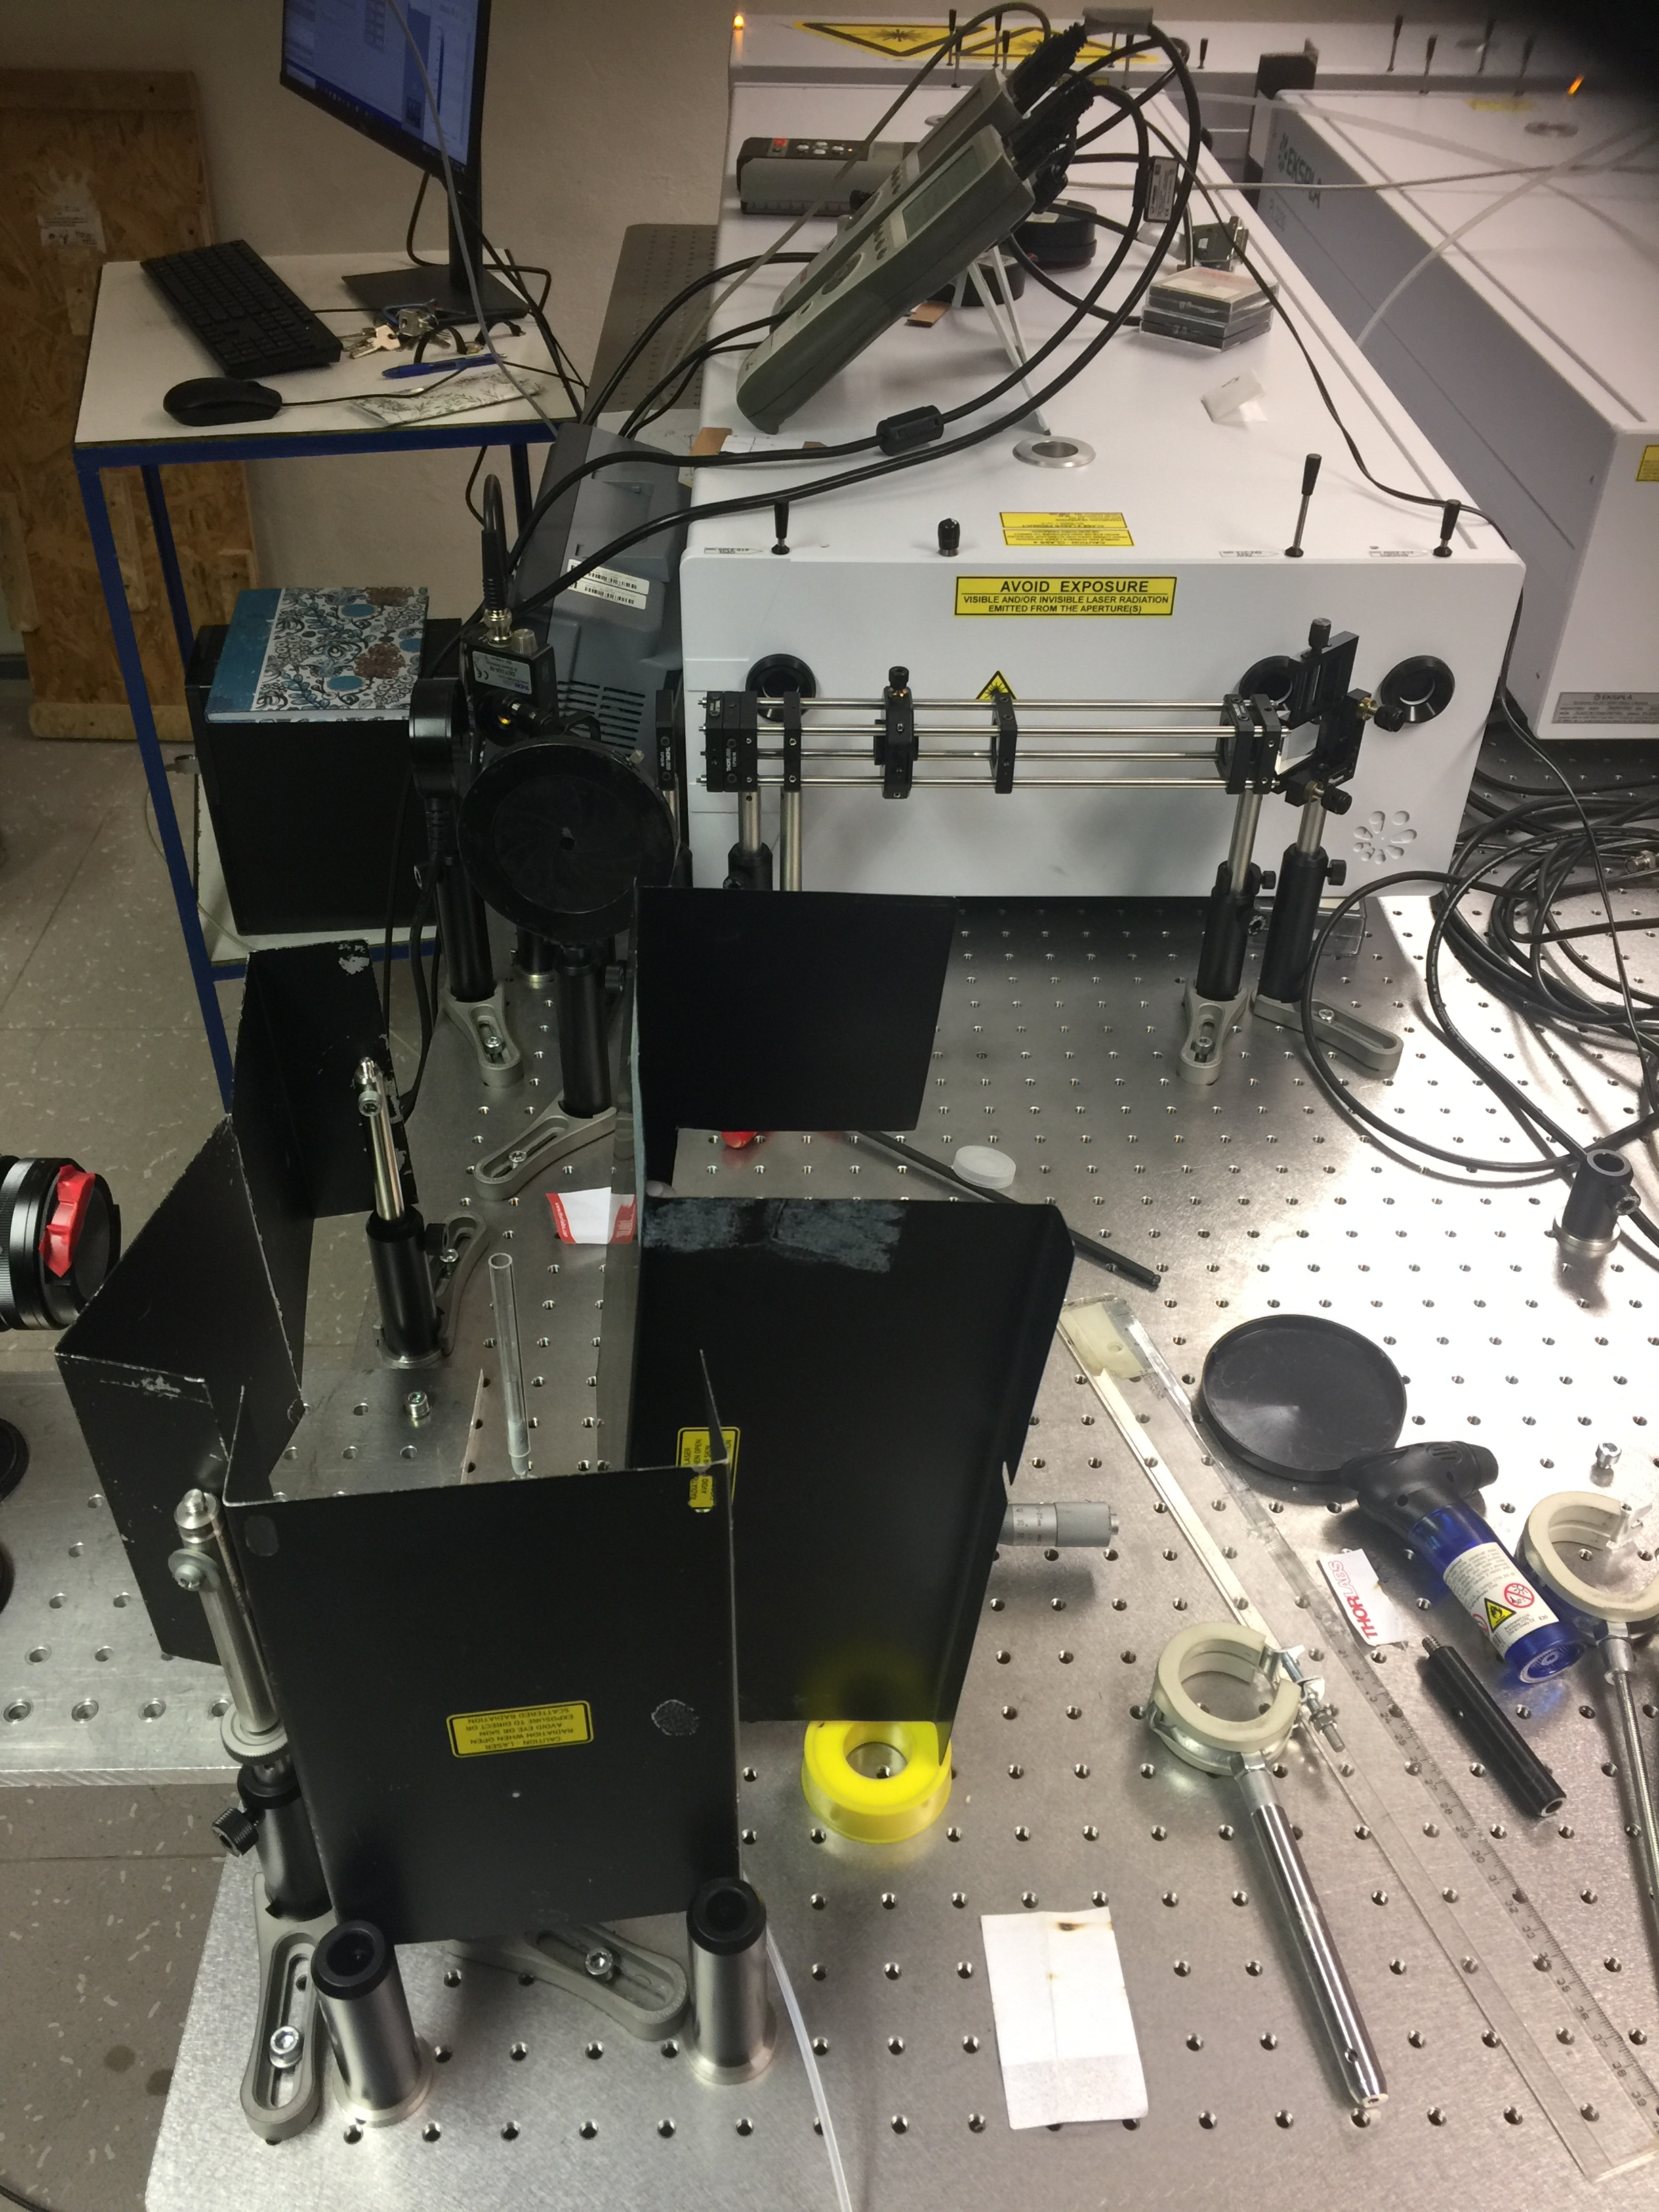
\includegraphics[width=\textwidth, trim={0 24 0 0}, clip]
		{img/lif-setup-photo-1}
	\caption{Snímek sestavené aparatury.
		Laserový svazek vychází druhým otvorem zprava,
		hned za hranolem je rám s~prostorovým filtrem.
		Dělič svazku je zčásti vidět za kruhovou clonou.
		Atomizátor je svislá skleněná trubička.
		Plechové zástěny rozmístěné v~okolí dráhy svazku
		slouží k~odstínění parazitního světla,
		zajištění tmavého pozadí a~k~ochraně plamene před prouděním vzduchu.
		Měřič energie za atomizátorem není vidět, je skryt za nejbližší
		zástěnou.
		Zcela vlevo je vidět objektiv ICCD kamery s~připevněnými
		křemennými sklíčky místo filtru.}%
	\label{fig:lif-setup-photo}
\end{figure}

\section{Vyhodnocení}
\label{sec:lif-method}
Před stanovením koncentrace atomů selenu bylo nutno určit několik
dalších veličin, na nichž výpočet závisí.
Prostřednictvím Rayleighova rozptylu byl zjištěn profil laserového svazku,
který udává prostorové rozložení intenzity excitujícího záření.
Změření excitačního profilu umožnilo nalézt přesnější polohu maxima
fluorescenčního signálu
a~stanovit spektrální překryv laseru a~excitace $\specoverlap$.
Ukázalo se, že fluorescence i~navzdory nízké energii laserových pulzů
projevovala saturaci, kterou bylo tudíž nutno zahrnout do výpočtů.
Podstatným krokem bylo určení doby života zářivého stavu.

Záznam z~ICCD kamery tvoří časová posloupnost jednokanálových sním\-ků,
přičemž každý snímek je tvořen nastaveným počtem akumulací na čipu.
Kamera kromě fluorescence snímá také parazitní signál pocházející
ze zbytkového světla v~laboratoři nebo vlastního záření plamene.
Pro potlačení jejich nežádoucího vlivu
byly všechny snímky korigovány odečtením temného snímku změřeného
s~vypnutým laserem za jinak stejných podmínek a~nastavení.

Pro výpočty byla použita energie laserových pulzů změřená za~atomizátorem.
V~případech, kdy bylo k~dispozici pouze měření za děličem,
byla energie za atomizátorem dopočtena podle závislosti obou energií
v~ostatních měřeních.
% Pro výpočty byla použita energie laserových pulzů změřená za děličem.
Energie byla následně zprůměrována v~časových intervalech odpovídajících
jednotlivým snímkům kamery.
Hranice těchto intervalů byly odhadnuty ze~známé frekvence spouštění
kamery, počtu akumulací na čipu a~vyčítací prodlevy mezi sním\-ky.

Na obrázku č.~\ref{fig:lif-flame} je samotný plamen bez laserové excitace
zaznamenaný ICCD kamerou bez použití filtru.
Intenzita byla v~tomto případě velmi slabá
(plamen byl pouhým okem neviditelný),
snímek je výsledkem \num{10000} akumulací.

\begin{figure}[p]
	\centering
	\input{../lif/results/flame}
	\caption{Snímek plamene bez laseru.
		Kamera byla bez filtru a~nastavena na \num{10000} akumulací.}
	\label{fig:lif-flame}
\end{figure}

\subsection{Profil svazku}
\label{sec:lif-rayleigh}
Pro další vyhodnocení bylo nutno znát skutečný prostorový profil
laserového svazku v~oblasti atomizátoru.
K~jeho zjištění bylo použito slabého rozptylu laserového záření ve vzduchu.
Uspořádání pokusu bylo stejné, jako bylo popsáno výše,
jen atomizátor byl vypnut (neproudil do něj žádný plyn).
Kamera snímala laserový svazek z~boku, zaznamenaný signál byl v~tomto
případě tvořen především Rayleighovým rozptylem svazku na částicích vzduchu.
Příklad takového snímku je na obrázku č.~\ref{fig:lif-beam}.
Snímaná intenzita byla mnohem větší než u~prostého plamene,
uvedený příklad je ze \num{100} akumulací.

\begin{figure}[p]
	\centering
	\input{../lif/results/rayleigh-example}
	\caption{Snímek laserového paprsku ve vzduchu bez plamene.
		Pozorovaný signál je Rayleighův rozptyl.
		Kamera byla bez filtru a~nastavena na \num{100} akumulací.}
	\label{fig:lif-beam}
\end{figure}

\begin{figure}
	\centering
	\input{../lif/results/rayleigh-profile-s}%
	\hfill
	\input{../lif/results/rayleigh-profile-norm-s}
	\caption{Svislý profil laserového svazku pro různé energie pulzu
		určený pomocí Rayleighova rozptylu.
		V~grafu vlevo je změřená intenzita fluorescence sečtená
		ve směru osy $\xpos$.
		Je patrno, že profil je mírně závislý na nastavené energii,
		neboť poloha maximální intenzity se s~rostoucí energií posouvá
		vzhůru (v~grafu doleva).
		Tento posuv je lépe vidět v~pravém grafu, kde jsou profily
		vyhlazené a~normalizované na jedničku.
		Normalizované profily byly použity k~výpočtu svislého
		rozdělení intenzity laserového paprsku pro známé energie pulzu.}
	\label{fig:lif-rayleigh-profile}
\end{figure}

\begin{figure}
	\centerline{\input{../lif/results/rayleigh-time}}
	\caption{Časový vývoj Rayleighova rozptylu v~průběhu jednoho pulzu.
		Signál je integrován v~horizontálním směru (ve směry osy $x$).}
	\label{fig:lif-rayleigh-time}
\end{figure}

\subsection{Excitační profil}
\label{sec:lif-excitprof}
Excitační profil byl změřen postupným laděním laseru na vlnové délky
v~rozsahu \SIrange{195.95}{196.20}{\nano\metre}
s~krokem \SI{0.001}{\nano\metre}.
Pokus byl proveden pro několik energií laserového pulzu $\enlaser$,
jak s~prostorovým filtrem, tak bez něj.

Na základě takto změřeného profilu byla poloha maxima LIF předběžně
odhadnuta na \SI{196.032}{\nano\metre}.
Při dalších měřeních byla vlnová délka laseru na\-stavena na tuto hodnotu.

Naměřená data byla dále aproximována Voigtovým profilem pomocí
Le\-ven\-berg-Marquardtova algoritmu.
Detail proložených profilů pro různé energie pulzu s~prostorovým filtrem
je na obrázku č.~\ref{fig:lif-excitprof-fit}
a~optimalizované parametry jsou v~tabulce č.~\ref{tab:lif-excitprof-fit}.

\begin{figure}
	\centering
	\input{../lif/results/excitprof-nofilter}
	\bigskip\par
	\input{../lif/results/excitprof-filter}
	\caption{Excitační profil bez prostorového filtru (nahoře)
		a~s~prostorovým filtrem (dole) pro několik energií pulzu.}
	\label{fig:lif-excitprof-filter}
\end{figure}

\begin{figure}
	\centering
	\input{../lif/results/excitprof-fit}
	\caption{Detail maxima integrálního excitačního profilu
		změřeného s~prostorovým filtrem
		a~spočtených aproximací Voigtovým profilem.}
	\label{fig:lif-excitprof-fit}
\end{figure}

\shorthandoff{-}
\begin{table}[bh]
	\centering
	\caption{Parametry aproximovaných excitačních profilů.
		$\enlaser$ je energie laserového pulzu,
		$\wavelen_\mathrm{max}$ je střed profilu,
		$\voigtsigma$ a~$\voigtgamma$ jsou šířky Gaussova a~Lorentzova profilu
		a~$\sum\Delta\lif^{2}$ je reziduální suma čtverců.}
	\label{tab:lif-excitprof-fit}
	\sisetup{
		table-alignment-mode = format,
		table-number-alignment = center,
	}
	\pgfplotstabletypeset[
		header = false,
		col sep = tab,
		skip first n = 1,
		every head row/.style = {
			before row = \toprule,
			after row = {
				\midrule
			}
		},
		string type,
		columns = {[index] 0, [index] 1, [index] 2, [index] 3, [index] 4},
		skip rows between index = {0}{5},
		columns/0/.style = {
			column name = $\enlaser\ [\si{\micro\joule}]$,
			column type = {S[
				table-format = 1.2,
				round-mode = places,
				round-precision = 2
			]},
		},
		columns/1/.style = {
			column name = $\wavelen_\mathrm{max}\ [\si{\nano\metre}]$,
			column type = {S[
				table-format = 3.4,
				round-mode = places,
				round-precision = 4
			]},
		},
		columns/2/.style = {
			column name = $\voigtsigma\ [\si{\nano\metre}]$,
			column type = {S[
				table-format = 1.4,
				round-mode = places,
				round-precision = 4
			]},
		},
		columns/3/.style = {
			column name = $\voigtgamma\ [\si{\nano\metre}]$,
			column type = {S[
				table-format = 1.4,
				round-mode = places,
				round-precision = 4
			]},
		},
		columns/4/.style = {
			column name = $\sum\Delta\lif^{2}$,
			column type = {S[
				table-format = 3.2,
				round-mode = places,
				round-precision = 2
			]},
		},
		every last row/.style = {after row = \bottomrule}
	]{../lif/results/excitprof-fit.tsv}
\end{table}
\shorthandon{-}

\subsection{Saturace}
\label{sec:lif-saturation}
Fluorescence podle očekávání vykazovala při použití vyšších intenzit laseru
znám\-ky saturace.
Jelikož tento jev nebyl zanedbatelný, bylo nutno jej vyšetřit,
aby jeho vliv mohl být zohledněn při stanovení koncentrace.

Laserový svazek měl v~místě plamene rovinný nerozbíhavý tvar
o~tloušťce asi \SI{1}{\milli\metre}.
Teoretická závislost LIF v~rovinném svazku při pozorování zboku
byla odvozena v~\cite{lif-pb}, kde je vyjádřena přibližným vztahem:
\begin{equation}
	\label{eq:lif-saturation}
	\lif(\enlasery) = \frac{2\lifslope}{\lifsat}
	\left( 1 - \frac{\ln(1 + \lifsat\enlasery)}{\lifsat\enlasery} \right).
\end{equation}
Zde $\lif$ je intenzita signálu LIF,
$\enlasery$ je intenzita laserového svazku ve výšce $\ypos$
(předpokládá se vodorovné vedení svazku),
a~$\lifslope$, $\lifsat$ jsou neznámé parametry.
Parametr $\lifslope$ popisuje lineární část závislosti pro velmi nízké energie,
parametr $\lifsat$ se nazývá saturační parametr a~udává zakřivení
závislosti v~nasycené oblasti.

Vlnová délka laseru byla držena na konstantní
hodnotě \SI{196.032}{\nano\metre},
zatímco energie pulzu byla postupně nastavována v~rozsahu
od zhruba \SI{0.5}{\micro\joule} do \SI{4.0}{\micro\joule}.

Kvůli rozsahům použitých měřičů bylo nutno měření rozdělit do dvou sérií:
první od \SI{2.0}{\micro\joule} do \SI{4.0}{\micro\joule}
a~druhé od \SI{0.5}{\micro\joule} do \SI{2.0}{\micro\joule}.
Při vyhodnocení se však ukázalo, že data z~obou sérií pro určité místo
ve výboji na sebe nenavazují plynule a~je mezi nimi patrný skok.
Obrázek \ref{fig:lif-saturation-full-example} toto chování ilustruje.
Jako možné vysvětlení se nabízí proměnlivost profilu laserového svazku
při změnách celkové energie pulzu, kterou ani prostorový filtr
nedokázal potlačit úplně.
Tato proměnlivost byla prokázána měřením rozptylu svazku ve~vzduchu,
jak ukazuje obrázek č.~\ref{fig:lif-rayleigh-profile}.

\begin{figure}
	\centering
	\input{../lif/results/saturation-full-example-index}
	\input{../lif/results/saturation-full-example-1}%
	\input{../lif/results/saturation-full-example-2}
	\input{../lif/results/saturation-full-example-3}%
	\input{../lif/results/saturation-full-example-4}
	\caption{Příklad dat z~měření saturace pro několik vybraných bodů.
		Přehledový snímek odpovídá energii pulzu \SI{3.99}{\micro\joule}.
		Níže jsou průběhy signálu $\lif$ v~závislosti na energii
		laseru $\enlaser$.
		Hodnoty $\lif$ v~nižším a~vyšším intervalu energií na sebe
		dobře nenavazují a~je mezi nimi patrný jistý skok,
		který znesnadňuje proložení předpokládanou
		závislostí \eqref{eq:lif-saturation}.
		Tento nesoulad je způsoben změnou svislého rozložení intenzity
		laserového svazku při změně celkové energie pulzu.}
	\label{fig:lif-saturation-full-example}
\end{figure}

Určení prostorově rozlišené saturace z~těchto dat se potýkalo s~obtížemi.
Bylo nutno důkladně zohlednit prostorovou variabilitu intenzity svazku.
Z~měření Rayleighova rozptylu svazku ve vzduchu byly k~dispozici
profily svazku naměřené pro čtyři různé celkové energie pulzu,
tyto profily jsou na obrázku \ref{fig:lif-rayleigh-profile} vlevo.

Profily byly pro odstranění šumu vyhlazeny klouzavým průměrem
a~odečtením pozadí.
Pak byly normovány na hodnotu 1 podle vztahu:
\begin{equation}
	\enlaserynorm = \frac{\enlasery}{\int \enlasery \mathrm{d}y},
\end{equation}
což je vidět na obrázku \ref{fig:lif-rayleigh-profile} vpravo.
Normované profily pro mezilehlé energie byly získány lineární interpolací
mezi naměřenými profily (lineární interpolace zachovává normovanost).
Profil intenzity v~každém snímku byl spočten vynásobením příslušného
normovaného profilu celkovou energií pulzu.
Výsledný průběh intenzit je na obrázku
č.~\ref{fig:lif-saturation-full-profile}.

\begin{figure}[htp]
	\centering
	\input{../lif/results/saturation-full-profile}
	\caption{Profil laserového svazku pro různé energie pulzu,
		integrovaný ve směru osy $\xpos$.
		Červené křivky jsou naměřené profily,
		modré křivky byly interpolovány z~naměřených.
		Každá interpolovaná křivka přísluší jednomu snímku kamery.
		Je zřetelný posuv maxima intenzity k~nižším hodnotám $\ypos$
		s~rostoucí energií.}
	\label{fig:lif-saturation-full-profile}
\end{figure}

Závislost intenzity fluorescence $\lif$ na energii laseru $\enlaser$
byla aproximována funkcí \eqref{eq:lif-saturation} pomocí metody
nejmenších čtverců, čímž byly získány parametry $\lifslope$ a~$\lifsat$.
Toto vyhodnocení bylo provedeno zvlášť pro každý pixel snímku,
přičemž každý snímek byl za účelem potlačení šumu vyhlazen klouzavým
průměrem ve čtverci o~rozměru \num{5}\times\SI{5}\pixel.

Spočtené hodnoty intenzitního parametru $\lifslope$ a~saturačního
parametru $\lifsat$ jsou na obrázku~\ref{fig:lif-saturation-full-params}
spolu s~ukázkou aproximovaných průběhů.
Je vidět, že parametr $\lifslope$ je soustředěn do centrální oblasti
nad atomizátorem, zatímco jinde jsou jeho hodnoty velmi nízké.
Za povšimnutí stojí, že směrem vzhůru roste, navzdory předpokladu,
že bude výraznější v~nižší části plamene.

Saturační parametr $\lifsat$ vykazuje při aproximaci větší nestabilitu
a~jeho hodnoty i~rozložení výrazně závisely na provedené korekci profilu
intenzity svazku $\enlasery$.
Na obrázku je jeho hodnota v~oblasti plamene zhruba homogenní:
Je sice patrn nárůst s~rostoucí výškou, stejně jako u~parametru $\lifslope$,
ale ve vodorovném směru se jeví stabilní.

\begin{figure}
	\centering
	\small
	\input{../lif/results/saturation-full-paramsfits}
	\caption{Parametry fluorescence $\lifslope$ a~$\lifsat$
		určené z~korigovaných hodnot energie
		a~příklad aproximovaných závislostí pro několik pixelů.
		Pro potlačení šumu byly snímky z~kamery před zpracováním vyhlazeny
		průměrováním ve čtverci o~rozměrech \num{5}\times\SI{5}{\pixel}.
		Je patrno, že saturační parametr $\lifsat$ je
		v~oblasti plamene ve vodorovném směru přibližně homogenní.}
	\label{fig:lif-saturation-full-params}
\end{figure}

Je nutno zdůraznit silnou závislost vypočteného saturačního parametru
na předpokládaném profilu laserového svazku.
Obrázek \ref{fig:lif-saturation-full-params-bad} ukazuje extrémní případ,
kdy byla k~vyhodnocení použita vždy jen jedna sada měření ze dvou.
První sada používala vyšší energie pulzu a~intenzita svazku byla soustředěna
více nahoře, druhá sada se pohybovala v~nízkých energiích
(zhruba do \SI{2}{\micro\joule}) a~největší intenzita svazku se nacházela níže.
Jak je z~obrázků patrno, výsledky se zásadně liší.
U~parametru $\lifslope$ je zachována vodorovná homogenita,
ale výškové rozdělení je zcela jiné.
U~saturačního parametru $\lifsat$ jakákoli rovnoměrnost zcela vymizela.

\begin{figure}[htp]
	\centering
	\small
	\input{../lif/results/saturation-full-params-bad}
	\caption{Ukázka nevhodného vyhodnocení parametrů $\lifslope$ a~$\lifsat$
		jako důkaz toho, že výsledky jsou velice citlivé na korekci intenzit.
		Nahoře jsou parametry spočítané z~datové sady vyšších energií,
		dole ze~sady nižších energií, kde je intenzita laseru soustředěna níže.
		Je vidět, že uvažovaný profil laserového svazku má značný vliv
		na výsledky.
		Zatímco parametr $\lifslope$ zůstává alespoň ve vodorovném směru
		homogenní, o~parametru $\lifsat$ nelze nic takového říci.
		Posun maxima intenzity směrem vzhůru navíc silně nadhodnocuje
		horní část snímané oblasti oproti dolní (viz grafy nahoře).}
	\label{fig:lif-saturation-full-params-bad}
\end{figure}

Alternativou k~výše uvedenému postupu je svislé rozlišení vůbec neuvažovat
a~obě veličiny, to jest intenzitu fluorescence $\lif$ i~intenzitu
laseru $\enlasery$, integrovat ve směry $\ypos$.
(V~případě intenzity laserového svazku to znamená vzít přímo
naměřenou hodnoty energie pulzu $\enlaser$.)
Obdobný postup, jako byl popsán výše, pak vede na vodorovně rozlišené
parametry $\lifslope$ a~$\lifsat$ na obrázku~\ref{fig:lif-saturation-x-params}.

\begin{figure}[htp]
	\centering
	\small
	\input{../lif/results/saturation-x-params}
	\caption{Parametry $\lifslope$ a~$\lifsat$ spočtené z~dat integrovaných
		ve směru svislé osy $\ypos$.
		Vodorovná čára označuje hodnotu $\lifsat$ spočítanou z~integrální
		intenzity celého snímku.
		Svislé čáry označují polohu ukázkových průběhů v~dolním obrázku.}
	\label{fig:lif-saturation-x-params}
	\bigskip
	\input{../lif/results/saturation-x-fits}
	\caption{Naměřená data pro vybrané polohy $\xpos$ a~spočtené proklady.
		Data v~nižším a~vyšším rozsahu energií na sebe dobře navazují,
		protože svislá proměnlivost profilu laserového svazku je skryta
		použitím celkové energie pulzu $\enlaser$.}
	\label{fig:lif-saturation-x-fits}
\end{figure}

\subsection{Doba života}
\label{sec:lif-lifetime}
Druhým významným ukazatelem koncentrace částic je doba života $\lifetime$,
tedy parametr exponenciálního poklesu signálu v~čase.
Časový vývoj fluorescence byl zaznamenán opakovaným měřením mnoha pulzů
s~postupně zvyšovaným zpožděním kamery za laserovým pulzem.
Délka každé expozice byla nastavena na \SI{2}{\nano\second},
po provedení 100 akumulací bylo vždy zpoždění kamery zvýšeno
o~\SI{0.5}{\nano\second}.
Takto byl zaznamenán časový interval o~délce \SI{30}{\nano\second}.
Atomizátor byl přitom nastaven na obvyklý průtok.

Série snímků na obrázku č.~\ref{fig:lif-timeev} ukazuje výběr několika
snímků z~tohoto měření.
Je vidět, že pulz, který dorazí zhruba v~čase $\SI{5}{\nano\second}$,
způsobí velmi rychlý nárůst fluorescence, která dosáhne maxima kolem
času $\SI{7}{\nano\second}$ a~poté výrazně pomaleji slábne.
Tímto poklesem intenzity byla proložena exponenciální funkce,
jejíž konstanta $\lifetime$ z~exponentu je doba života.

Spočtená doba života pro každý pixel středové oblasti snímku je
na obrázku \ref{fig:lif-lifetime-full-params}.
Je patrno, že ve~středu plamene je doba života nejvyšší
a~směrem k~okrajům slábne.
Vně plamene je signál velmi slabý a~spočtené hodnoty $\lifetime$
nejsou věrohodné.

Náročnost zpracování byla v~tomto případě výrazně nižší než u~saturace,
neboť doba života nezávisí na absolutní velikosti signálu
a~nebylo proto nutné provádět korekci na proměnlivost profilu
laserového svazku.
Ukázka prokládaných dat pro několik pixelů je
na obrázku~\ref{fig:lif-lifetime-full-params} dole.

\begin{figure}[p]
	\centering
	\input{../lif/results/timeev}
	\caption{Typický vývoj fluorescenčního signálu v~průběhu jedné periody.
		Časové rozlišení bylo získáno opakovaným měřením mnoha period
		s~postupnou změnou zpoždění kamery za začátkem pulzu.
		Pulz začíná přibližně v~čase $\tim = \SI{5.0}{\nano\second}$.
		Kamera byla ve všech snímcích nastavena na \num{100} akumulací.
		Hloubka snímané oblasti, daná tloušťkou laserového svazku,
		je zhruba \SI{1}{\milli\metre}.}
	\label{fig:lif-timeev}
\end{figure}

\begin{figure}[htp]
	\centering
	\input{../lif/results/lifetime-full-params}
	\input{../lif/results/lifetime-full-fits}
	\caption{Určená doba života $\lifetime$.
		Body po stranách obrázku jsou spočítané z~velmi malých hodnot
		signálu a~nejsou proto věrohodné.
		Níže je příklad proložených dat pro několik vybraných bodů.}
	\label{fig:lif-lifetime-full-params}
\end{figure}

Protože doba života v~plném rozlišení je značně zatížena šumem,
byla kromě ní spočtena i~doba života ze svisle integrovaných dat,
obdobně jako v~případě saturace.
Tato vodorovně rozlišená doba života je vykreslena
na obrázku~\ref{fig:lif-lifetime-x-params}.
Zde je jasně zřetelné, že její maximum leží zhruba ve středu plamene
a~směrem ke krajům klesá.
Pozoruhodné je, že závislost se zdá být velmi podobná lineární.
Ukázka prokladů ve vybraných bodech je
na obrázku~\ref{fig:lif-lifetime-x-fits}.
Zde je patrno, že svislá integrace signálu měla za následek potlačení šumu
a~tím pádem přesnější proklady.

\begin{figure}[htp]
	\centering
	\input{../lif/results/lifetime-x-params}
	\caption{Doba života $\lifetime$ určená z~dat integrovaných ve směru
		svislé osy $\ypos$.
		Barevné čáry označují polohu ukázkových průběhů níže.}
	\label{fig:lif-lifetime-x-params}
	\bigskip
	\input{../lif/results/lifetime-x-fits}
	\caption{Naměřená data integrovaná ve směry $\ypos$ a~proložený
		exponenciální pokles pro vybrané polohy $\xpos$.}
	\label{fig:lif-lifetime-x-fits}
\end{figure}

\subsection{Koncentrace atomů}
\label{sec:lif-concentration}

\begin{table}
	\centering
	\caption{Spektrální čáry selenu použité pro LIF a~jejich parametry.
		Sloupec $\transmittance$ je propustnost filtru před kamerou
		a~$\qeff$ je kvantová účinnost kamery.}
	\label{tab:lif-liflines}
	\sisetup{
		table-alignment-mode = format,
		table-number-alignment = center,
	}
	\pgfplotstabletypeset[
		outfile = log.tex,
		col sep = tab,
		every head row/.style = {
			before row = \toprule,
			after row = {
				\midrule
			}
		},
		every last row/.style = {after row = \bottomrule},
		string type,
		columns = {wl[nm], A32, T, eff},
		columns/{wl[nm]}/.style = {
			column name = $\wavelen\ [\si{\nano\metre}]$,
			column type = {S[
				table-format = 3.3,
				round-mode = places,
				round-precision = 3
			]},
		},
		columns/A32/.style = {
			column name = $\einsteina\ [\si{\per\second}]$,
			column type = {S[
				exponent-mode = scientific,
				table-format = 1.2e2,
				round-mode = places,
				round-precision = 2,
			]},
		},
		columns/B23/.style = {
			column name = $\einsteinb$,
			column type = {S[
				exponent-mode = scientific,
				table-format = 1.2e2,
				round-mode = places,
				round-precision = 2,
			]},
		},
		columns/T/.style = {
			column name = $\transmittance$,
			column type = {S[
				table-format = 1.3,
				round-mode = places,
				round-precision = 3,
			]},
		},
		columns/eff/.style = {
			column name = $\qeff$,
			column type = {S[
				table-format = 1.3,
				round-mode = places,
				round-precision = 3,
			]},
		},
	]{../lif/results/liflines.tsv}
\end{table}

\section{Výsledky}
\label{sec:lif-results}

\begin{figure}[htp]
	\centering
	\input{../lif/results/concentration-single}
	\caption{Hustota atomů selenu určená ze snímku
		s~maximální energií laserového pulzu $\enlaser$.}
	\label{fig:lif-concentration-single}
\end{figure}

\begin{figure}[htp]
	\centering
	\input{../lif/results/concentration-mean}
	\input{../lif/results/concentration-std}
	\caption{Hustota atomů selenu jako průměr ze všech snímků
		a~její nejistota spočtená jako směrodatná odchylka.}
	\label{fig:lif-concentration-mean}
\end{figure}

\begin{figure}[htp]
	\centering
	\input{../lif/results/concentration-vertical-700+300}
	\caption{Prostorově rozlišená hustota atomů selenu v~plameni.
		Koláž 15 snímků v~různých výškách.}
	\label{fig:lif-vertical-concentration-700+300}
\end{figure}

% {\graphicspath{{../talif/}{build/epstopdf}{img/}}\chapter[TALIF]{Dvoufotonová laserem indukovaná fluorescence kryptonu}
\label{sec:talif}

\providecommand\xpos{x}
\providecommand\ypos{y}
\providecommand\xmm{x}
\providecommand\ymm{y}

\begin{figure}[htp]
	\centering
	\input{../talif/results/lifetime-x-params}
	\caption{Doba života $\lifetime$ určená z~dat integrovaných ve směru
		svislé osy $\ypos$.
		Čárkovaná čára označuje polohu ukázkových průběhů níže.}
	\label{fig:talif-lifetime-x-params}
	\bigskip
	\input{../talif/results/lifetime-x-fits}
	\caption{Naměřená data integrovaná ve směry $\ypos$ a~proložený
		exponenciální pokles pro vybrané polohy $\xpos$.}
	\label{fig:talif-lifetime-x-fits}
\end{figure}
}
% TODO: Závěr

\backmatter
\printbibliography[heading=bibintoc,title=Seznam použité literatury]
\label{lastpage}

\end{document}
